\chapter{Introduction}
\label{cha:introduction}

To detect brain tumours and classify them into malignant and benign, is a vital challenge in the field of medical diagnostics. 
Accurate and timely diagnosis is essential for effective treatment planning and improving the patient's health.
Traditional methods for diagnosing brain tumours are biopsies or manually evaluating medical images like magnetic resonance imaging (MRI) scans \cite{CancerResearUK}.
These methods are time-consuming, expensive, and can be error-prone. 
With advancements in the field of machine learning, it is possible to automate the process of diagnosing brain tumours using machine learning techniques. %convolutional neural networks (CNNs).
To use machine learning, the brain tumour which is to be classified as malignant or benign, needs to be analysed by a doctor into certain features.
These features can be extracted from MRI scans and used as input for a machine-learning model.
To overcome this analysis step by maybe even multiple doctors, a neural network can be trained on the MRI scans themselves.
A task such as this is known as image classification.
Convolutional neural networks (CNNs) are a type of artificial neural network that is well-suited for image classification tasks, by applying filters to input images to detect patterns.

In this work, we aim to develop a CNN to classify brain tumours in MRI scans as malignant or benign.
This model is compared to binary classification models to evaluate its performance, such as logistic regression, support vector machines, and k-nearest neighbours.
The metric used to evaluate the models is the recall score, as it is important to detect malignant tumours correctly.

The dataset used in this work is the "Brain Tumor" dataset from Kaggle \cite{jakesh_bohaju_2020}.
It contains 3762 images with labels that can be used for the CNN.
It also contains five first-order and eight second-order features that can be used for the binary classification methods.
The first-order features are mean, variance, skewness, kurtosis, and entropy.
The second-order features are contrast, energy, angular second moment (ASM), entropy, homogeneity, dissimilarity, correlation, and coarseness.
The dataset runs under the Creative Commons license, which allows for sharing and adapting the dataset for non-commercial purposes \href{https://creativecommons.org/licenses/by-nc-sa/4.0/}{(CC BY-NC-SA 4.0)}. 
The CNN is trained on the images from the dataset, and the binary classification models are trained on the features extracted from the images.

The CNN is explained in more detail in chapter \ref{cha:CNN}, where the network architecture, the initial model, the hyperparameter optimization, and the final model are discussed.
The binary classification models are explained in chapter \ref{cha:alternative_methods}.
A comparison between the CNN and the binary classification models is made in section \ref{sec:comparison}.
A discussion and an outlook are given in chapter \ref{cha:conclusion}.

% \section{Dataset}
% \label{sec:dataset}



% \cite{tensorflow}
% \begin{figure}[H]
%     \centering
%     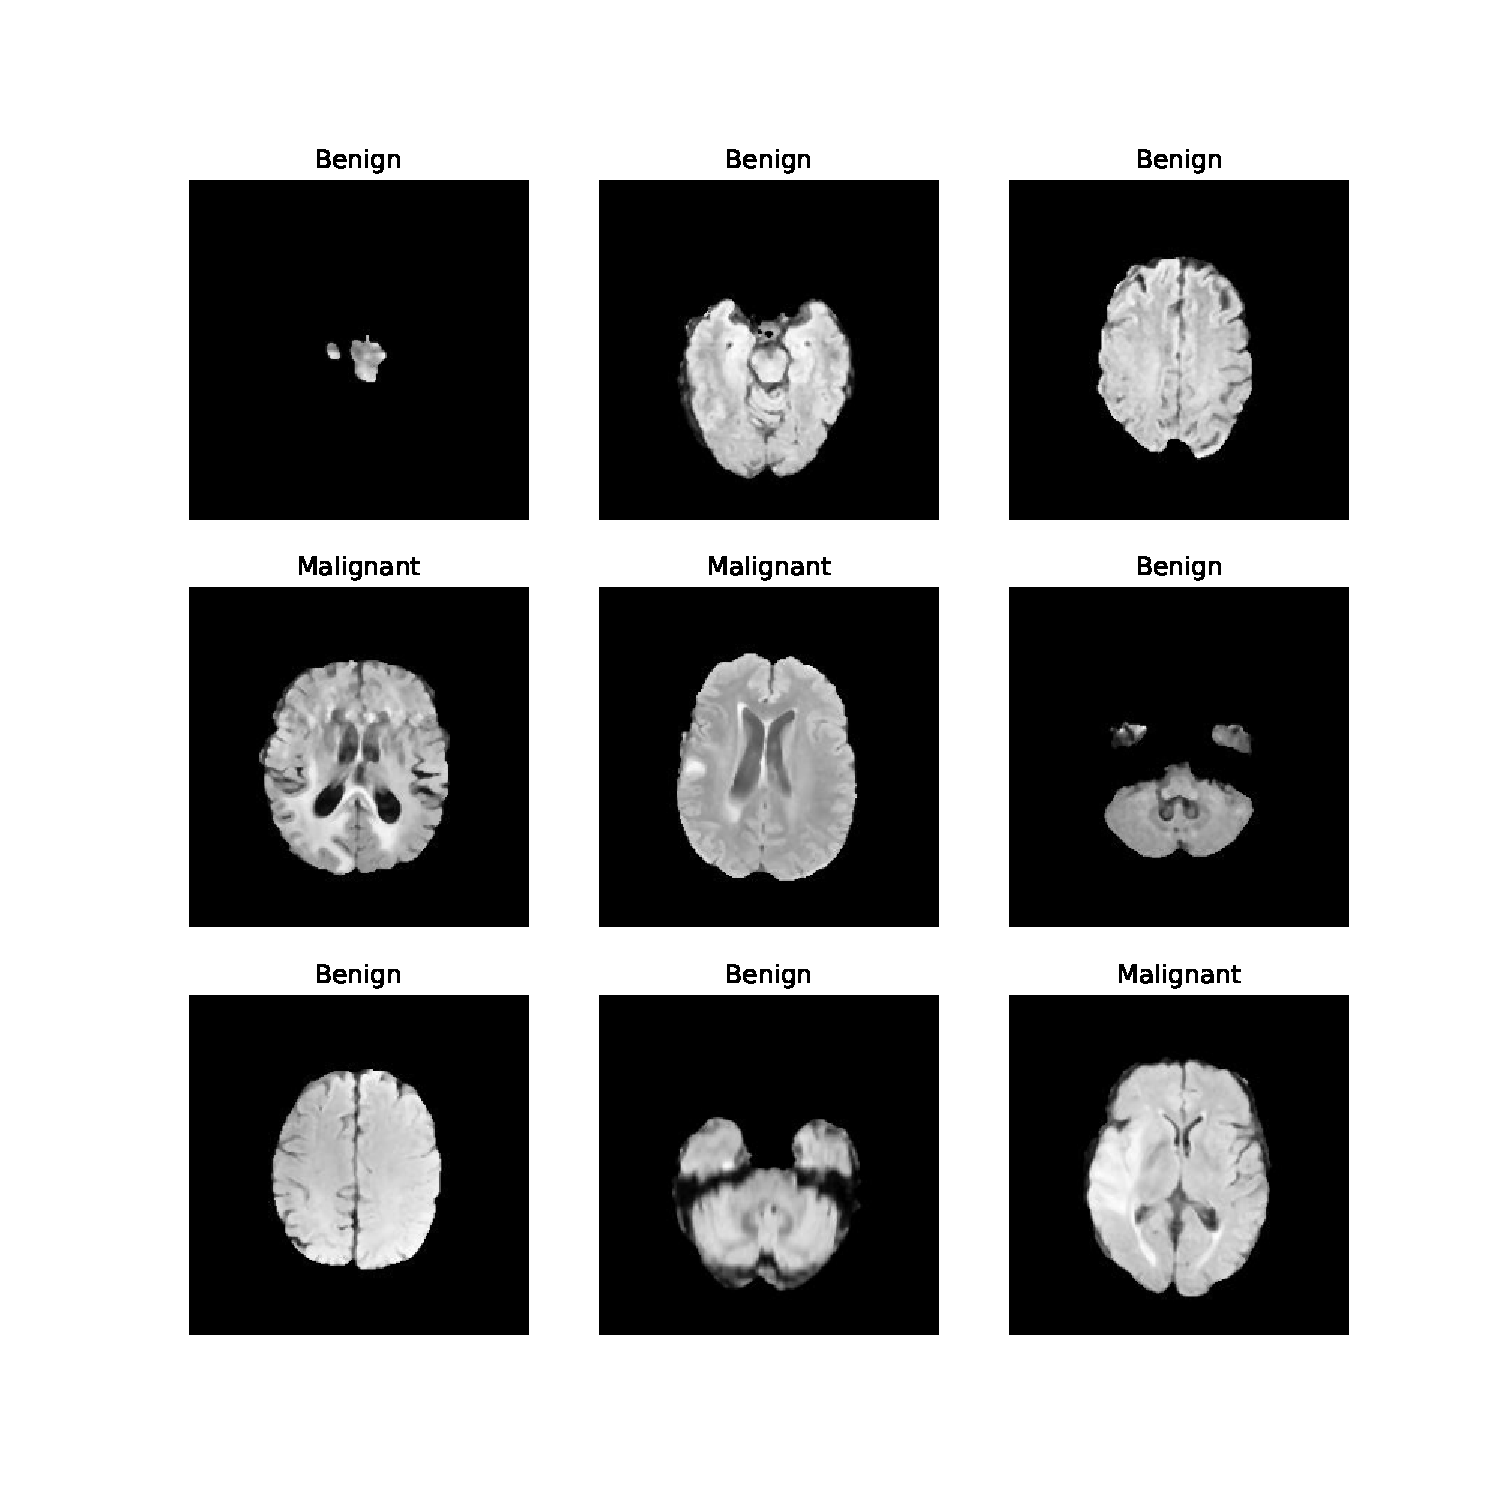
\includegraphics[width=.8\textwidth]{plots/tumor_images.pdf}
%     \caption{Malignant and benign tumour images from the dataset.}
%     \label{fig:tumorImages}
% \end{figure}
